%% ──────────────────────────────────────────────────────────────────
%%  Diabetic Retinopathy — Lab 5 Report
%%  Computer Vision, April 2026
%% ──────────────────────────────────────────────────────────────────
\documentclass[a4paper, 10pt, twocolumn]{article}

\usepackage[top=1.8cm, bottom=1.8cm, left=1.4cm, right=1.4cm, columnsep=0.65cm]{geometry}
\usepackage[utf8]{inputenc}
\usepackage[T1]{fontenc}
\usepackage{lmodern}
\usepackage{microtype}
\usepackage{booktabs}
\usepackage{multirow}
\usepackage{pgfplots}
\pgfplotsset{compat=1.18}
\usepackage{xcolor}
\usepackage{titlesec}
\usepackage[hidelinks]{hyperref}
\usepackage{enumitem}
\usepackage{amsmath}
\usepackage[labelfont=bf, font=small, skip=3pt]{caption}
\usepackage{tabularx}
\usepackage{graphicx}

%% ── Colour palette ────────────────────────────────────────────────
\definecolor{accent}{RGB}{0, 64, 128}
\definecolor{rowbest}{RGB}{220, 240, 220}
\definecolor{rowbad} {RGB}{255, 230, 230}
\definecolor{rownorm}{RGB}{250, 250, 252}
\definecolor{rulecolor}{RGB}{0, 64, 128}

%% ── Section headings ─────────────────────────────────────────────
\titleformat{\section}
  {\normalfont\bfseries\small\color{accent}}
  {}{0em}{}[{\color{rulecolor}\vspace{-1pt}\hrule height 0.6pt\vspace{1pt}}]
\titlespacing{\section}{0pt}{6pt}{2pt}

\titleformat{\subsection}
  {\normalfont\small\bfseries}
  {}{0em}{}
\titlespacing{\subsection}{0pt}{3pt}{1pt}

%% ── Paragraph / list style ───────────────────────────────────────
\setlength{\parskip}{2pt}
\setlength{\parindent}{0pt}
\setlist[itemize]{topsep=1pt, itemsep=0pt, leftmargin=10pt,
                  label=\raisebox{0.3ex}{\tiny$\bullet$}, parsep=0pt}

%% ── Captions ─────────────────────────────────────────────────────
\setlength{\abovecaptionskip}{3pt}
\setlength{\belowcaptionskip}{0pt}

%% ══════════════════════════════════════════════════════════════════
\begin{document}

%% ── Title spanning both columns ──────────────────────────────────
\twocolumn[{%
\begin{center}
  {\large\bfseries\color{accent}
    Automatic Diagnosis of Diabetic Retinopathy\\[2pt]
    via Custom CNN Architecture and Transfer Learning}\\[4pt]
  {\small
    Maria Muñoz Pérez \enspace$\cdot$\enspace
    Cristina [Surname]\enspace$\cdot$\enspace
    Computer Vision --- Lab 5 \enspace$\cdot$\enspace April 2026}\\[3pt]
  {\color{rulecolor}\hrule height 0.8pt}
  \vspace{5pt}
\end{center}
}]

%% ── 1. INTRODUCTION ──────────────────────────────────────────────
\section{Introduction}

Diabetic Retinopathy (DR) is a leading cause of preventable blindness.
This work develops a binary DR/No-DR classifier from fundus photographs
across two competition tracks: a \emph{custom} CNN trained from scratch
(CUSTOM) and a \emph{fine-tuned} pretrained backbone (FINE-TUNING).
Performance is measured by AUC on a held-out 1\,000-image test set
evaluated via Codabench.

%% ── 2. DATASET & PREPROCESSING ──────────────────────────────────
\section{Dataset \& Preprocessing}

The dataset contains 2\,000 training / 500 validation / 1\,000 test fundus
images with a severe class imbalance (73\% No-DR, 27\% DR). Right-eye
images are horizontally mirrored to unify anatomical orientation.

\textbf{Pipeline.}
A threshold-based \texttt{CropByEye} transform crops the visible retinal
disc, removing black borders. Images are rescaled to 256\,px; training
augmentations add random horizontal flip, rotation ($\pm$15°), colour
jitter, and a random 224\,px crop. Validation uses a deterministic centre
crop. All images are ImageNet-normalised
($\mu$=[0.485,\,0.456,\,0.406]; $\sigma$=[0.229,\,0.224,\,0.225]).

%% ── 3. CUSTOM MODEL ──────────────────────────────────────────────
\section{Custom Model (CUSTOM)}

\subsection{Baseline: CustomNet}
A 4-block CNN with 5$\times$5 no-padding convolutions
(3→6→16→32→64), BatchNorm and MaxPool per block, flattened to 6\,400-d,
and head 6400→120→84→\texttt{Dropout}(0.5)→1. SGD + StepLR; AUC\,=\,0.570.

\subsection{CustomNetV2}
To improve generalisation on the small training set:
\begin{itemize}
  \item \textbf{5 blocks, 3$\times$3 same-padding} convolutions
        (3→32→64→128→256→256), reducing spatial size with MaxPool per block.
  \item \textbf{Global Average Pooling} replaces the 6\,400-d flatten,
        giving translation invariance and a compact 256-d representation.
  \item \textbf{Head}: \texttt{Dropout}(0.2)→Linear(256,128)→ReLU→
        \texttt{Dropout}(0.4)→Linear(128,1).
  \item \textbf{Optimiser}: AdamW (lr=1e-3, wd=5e-3),
        CosineAnnealingLR ($T_\text{max}$=50), 50\,epochs, patience=10.
\end{itemize}
Adding \texttt{WeightedRandomSampler} raises public AUC from 0.744 to
\textbf{0.766} (+34\% over baseline).

%% ── 4. FINE-TUNING MODEL ─────────────────────────────────────────
\section{Fine-tuning Model (FINE-TUNING)}

\subsection{Backbone: EfficientNet-B0}
ResNet18~\cite{he2016deep} yielded 0.698 AUC. We switched to
\textbf{EfficientNet-B0}~\cite{tan2019efficientnet} (ImageNet top-1
77.1\%), replacing its classifier with \texttt{Dropout}(0.3)→Linear(1280,1).
Unfreezing only \texttt{features[6--8]} plus the new head (3.16\,M of
4.01\,M parameters), with AdamW~\cite{loshchilov2019adamw} (lr=3e-4,
wd=1e-2) and CosineAnnealingLR ($T_\text{max}$=30) for 30\,epochs, raised
AUC to 0.751.

\subsection{Two-Stage Progressive Unfreezing}
Fine-tuning all layers on 2\,000 images risks overfitting.
\emph{Stage~1} trains only deep blocks (\texttt{features[6--8]}) + head.
\emph{Stage~2} additionally unfreezes \texttt{features[5]} at lr=3e-5,
triggered only if Stage~1 TTA AUC\,$\geq$\,0.752; Stage~1 weights are
restored if Stage~2 regresses. Despite this, overfitting persists: train
AUC reaches 0.957 at the best val checkpoint with a 0.178 train--val gap
(Fig.~\ref{fig:curves}).

%% ── 5. TRAINING OPTIMIZATIONS ────────────────────────────────────
\section{Training Optimizations}

\textbf{Class-imbalance handling.}
\texttt{BCEWithLogitsLoss} with \texttt{pos\_weight}\,$\approx$\,2.76
addresses imbalance at the gradient level. \texttt{WeightedRandomSampler}
oversamples the minority class at the mini-batch level ($+$0.022\,AUC).

\textbf{Test-Time Augmentation (TTA).}
Scores are averaged over the original and horizontally-flipped image
(+0.008--0.012\,AUC, applied at inference only).

\textbf{Label Smoothing.}
For EfficientNet only ($\varepsilon$=0.05), hard targets become soft
$\{0.025, 0.975\}$, penalising overconfident logits without damaging the
limited training signal on a small dataset~\cite{muller2019label}.

\textbf{Ensemble.}
A grid search over $w\in\{0.10,\ldots,0.30\}$ on validation selects the
optimal blend of CustomNetV2 and EfficientNet scores. A val--test gap of
$\approx$0.02--0.03\,AUC is consistently observed
(val\,0.796\,$\to$\,public\,0.770).

%% ── 6. ABLATIONS & NEGATIVE RESULTS ─────────────────────────────
\section{Ablations \& Negative Results}

\begin{itemize}
  \item \textbf{CLAHE preprocessing}: histogram equalisation before
    \texttt{CropByEye} broke its intensity threshold, dropping custom
    AUC by 4.6\% (0.570→0.544).
  \item \textbf{Cache pipeline}: pre-computing fixed 224\,px crops
    removed per-epoch \texttt{RandomCrop} spatial jitter — a key
    regulariser on 2\,000 images — costing $-$0.028\,AUC despite a 5$\times$
    speed-up.
  \item \textbf{Scale jitter (TVRandomResizedCrop)}: no consistent gain
    ($-$0.004 vs best).
  \item \textbf{BenGraham preprocessing}: local contrast normalisation
    caused catastrophic collapse (custom 0.541, ft 0.558) due to a dtype
    bug: the transform assumed float [0,1] input but received uint8 [0,255]
    from \texttt{CropByEye}. \texttt{clip(uint8,0,1)} mapped all pixels to
    $\{0,1\}$; the contrast formula produced uniform grey images, making
    every training sample indistinguishable.
\end{itemize}

%% ── 7. INDIVIDUAL CONTRIBUTIONS ─────────────────────────────────
\section{Individual Contributions}

\textbf{Cristina [Surname]:} Baseline exploration in
\texttt{first\_attempt.ipynb} — class-imbalance analysis, CustomNet
design, initial data pipeline, and first Codabench submission.

\textbf{Maria Muñoz:} All subsequent work (experiments B–H) —
CustomNetV2 design, EfficientNet-B0 two-stage fine-tuning, Weighted\-Random\-Sampler, TTA, ensemble grid search, label smoothing,
scale-jitter and cache ablations, and all notebook documentation.

%% ══════════════════════════════════════════════════════════════════
%% PAGE 2 — TABLES, FIGURES & REFERENCES
%% ══════════════════════════════════════════════════════════════════
\newpage
\onecolumn

\section*{\color{accent}Supplementary Material: Tables, Figures and References}
{\color{rulecolor}\hrule height 0.6pt}
\vspace{8pt}

%% ── TABLE 1 (full width) ──────────────────────────────────────────
\captionof{table}{%
  AUC results for all submitted experiments
  (\emph{pub}\,=\,public leaderboard, \emph{priv}\,=\,private).
  \textbf{Bold}: best result. \textit{Italic\,/\,red rows}: discarded experiment.}
\label{tab:results}
\vspace{3pt}
\footnotesize
\setlength{\tabcolsep}{5pt}
\renewcommand{\arraystretch}{1.22}
\begin{tabularx}{\textwidth}{@{}lXcc@{}}
\toprule
\textbf{Notebook} & \textbf{Key change(s)} &
  \textbf{Custom AUC} & \textbf{FT AUC} \\
 & & \scriptsize pub\;/\;priv & \scriptsize pub\;/\;priv \\
\midrule
\texttt{first\_attempt}         & CustomNet (baseline) + ResNet18 fine-tuning          & 0.570\;/\;0.597 & 0.698\;/\;0.708 \\
\texttt{attempt\_with\_b}       & CustomNet: Adam optimiser + CosineAnnealingLR        & 0.558\;/\;0.566 & 0.692\;/\;0.693 \\
\texttt{attempt\_with\_a\_b}    & \textcolor{red!70!black}{\textit{CLAHE preprocessing — broke CropByEye ($-$4.6\%)}} & \textcolor{red!70!black}{\textit{0.544\;/\;0.562}} & \textcolor{red!70!black}{\textit{0.711\;/\;0.692}} \\
\texttt{attempt\_with\_c}       & FT: switch to EfficientNet-B0 + AdamW                & 0.561\;/\;0.579 & 0.751\;/\;0.734 \\
\texttt{second\_attempt}        & CustomNetV2; 2-stage progressive FT; TTA; Ensemble   & 0.744\;/\;0.731 & 0.742\;/\;0.727 \\
\texttt{second\_attempt\_tuned} & \textcolor{accent}{\textbf{+ WeightedRandomSampler (balanced mini-batches)}} & \textcolor{accent}{\textbf{0.766\;/\;0.743}} & \textcolor{accent}{\textbf{0.770\;/\;0.744}} \\
\texttt{s.a.t.\_cache}          & \textcolor{red!70!black}{\textit{Cache pipeline — removes RandomCrop jitter ($-$0.028)}} & \textcolor{red!70!black}{\textit{0.736\;/\;0.730}} & \textcolor{red!70!black}{\textit{0.742\;/\;0.728}} \\
\texttt{third\_attempt}         & Scale jitter (ResizedCrop); label smoothing; $T_\mathrm{max}$=25 & 0.762\;/\;0.742 & 0.766\;/\;0.743 \\
\texttt{fourth\_attempt}        & \textcolor{red!70!black}{\textit{BenGraham — uint8 dtype bug, all images grey ($-$22\%)}} & \textcolor{red!70!black}{\textit{0.541\;/\;0.557}} & \textcolor{red!70!black}{\textit{0.558\;/\;0.533}} \\
\bottomrule
\end{tabularx}

\vspace{10pt}

%% ── TABLE 2 + FIGURE (side by side) ──────────────────────────────
\begin{minipage}[t]{0.47\textwidth}

\captionof{table}{Architecture and training comparison.}
\label{tab:arch}
\vspace{3pt}
\footnotesize
\setlength{\tabcolsep}{4pt}
\renewcommand{\arraystretch}{1.18}
\begin{tabular}{@{}lcc@{}}
\toprule
\textbf{Feature} & \textbf{CustomNet} & \textbf{CustomNetV2} \\
\midrule
Conv blocks  & 4 (5$\times$5, no-pad)    & 5 (3$\times$3, same-pad) \\
Channels     & 3$\to$6$\to$16$\to$32$\to$64 & 3$\to$32$\to$64$\to$128$\to$256$\to$256 \\
Spatial head & Flatten (6\,400-d)        & Glob.\ Avg Pool (256-d) \\
FC head      & 6400$\to$120$\to$84$\to$1 & 256$\to$128$\to$1 \\
Conv Bias    & Yes                       & No (BN absorbs) \\
Optimiser    & SGD                       & AdamW (wd=5e-3) \\
LR schedule  & StepLR ($\gamma$=0.1)    & CosineAnnealingLR \\
Sampler      & Uniform                   & Weighted (class) \\
\midrule
Public AUC   & 0.570                     & \textbf{0.766} \\
\bottomrule
\end{tabular}

\end{minipage}%
\hfill
\begin{minipage}[t]{0.50\textwidth}

%% ── FIGURE 1 ─────────────────────────────────────────────────────
\captionof{figure}{EfficientNet-B0 Stage\,1 training curves
(\texttt{second\_attempt\_tuned}). Train AUC reaches 0.957 at the
best val checkpoint ($\star$, epoch\,14) while val AUC peaks at 0.779,
revealing a gap of 0.178. This overfitting motivated label smoothing,
progressive unfreezing, and TTA.}
\label{fig:curves}
\vspace{3pt}

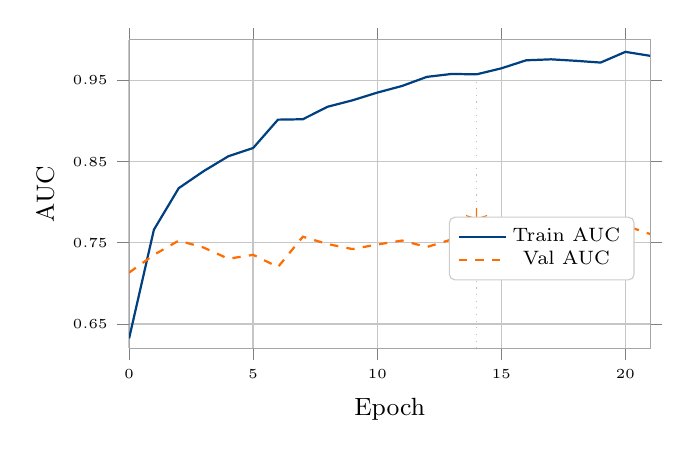
\begin{tikzpicture}
\begin{axis}[
  width  = 8.2cm,
  height = 5.5cm,
  xlabel = {Epoch},
  ylabel = {AUC},
  xmin=0, xmax=21,
  ymin=0.62, ymax=1.00,
  xtick={0,5,10,15,20},
  ytick={0.65,0.75,0.85,0.95},
  tick label style={font=\tiny},
  label style={font=\small},
  legend style={
    font=\scriptsize,
    at={(0.97,0.22)}, anchor=south east,
    draw=gray!40, fill=white, rounded corners=2pt,
    row sep=-2pt,
  },
  grid=both,
  grid style={line width=0.3pt, draw=gray!25},
  major grid style={line width=0.5pt, draw=gray!45},
  tick align=outside,
  axis line style={gray!70},
]

\addplot[color=accent, thick, mark=none] coordinates {
  (0,0.6322)(1,0.7661)(2,0.8172)(3,0.8381)(4,0.8565)
  (5,0.8667)(6,0.9016)(7,0.9021)(8,0.9175)(9,0.9254)
  (10,0.9349)(11,0.9431)(12,0.9543)(13,0.9579)(14,0.9574)
  (15,0.9648)(16,0.9747)(17,0.9759)(18,0.9741)(19,0.9719)
  (20,0.9851)(21,0.9802)
};
\addlegendentry{Train AUC}

\addplot[color=orange!85!red, thick, dashed, mark=none] coordinates {
  (0,0.7132)(1,0.7351)(2,0.7526)(3,0.7441)(4,0.7303)
  (5,0.7351)(6,0.7201)(7,0.7574)(8,0.7484)(9,0.7422)
  (10,0.7478)(11,0.7527)(12,0.7447)(13,0.7541)(14,0.7793)
  (15,0.7696)(16,0.7682)(17,0.7622)(18,0.7706)(19,0.7643)
  (20,0.7711)(21,0.7607)
};
\addlegendentry{Val AUC}

\addplot[only marks, mark=star, mark size=4pt, color=orange!85!red]
  coordinates { (14,0.7793) };
\addplot[gray!50, thin, dotted] coordinates { (14,0.62) (14,0.9574) };

\end{axis}
\end{tikzpicture}

\end{minipage}

\vspace{10pt}

%% ── REFERENCES ───────────────────────────────────────────────────
\renewcommand{\refname}{\normalfont\bfseries\small\color{accent}References}
\begin{thebibliography}{9}
\small\setlength{\itemsep}{1pt}

\bibitem{tan2019efficientnet}
Tan, M., \& Le, Q.\,V. (2019).
EfficientNet: Rethinking model scaling for convolutional neural networks.
\textit{Proc.\ ICML 2019}.

\bibitem{he2016deep}
He, K., Zhang, X., Ren, S., \& Sun, J. (2016).
Deep residual learning for image recognition.
\textit{Proc.\ CVPR 2016}, 770--778.

\bibitem{loshchilov2019adamw}
Loshchilov, I., \& Hutter, F. (2019).
Decoupled weight decay regularization.
\textit{Proc.\ ICLR 2019}.

\bibitem{muller2019label}
Müller, R., Kornblith, S., \& Hinton, G. (2019).
When does label smoothing help?
\textit{Proc.\ NeurIPS 2019}, 4694--4703.

\bibitem{graham2015kaggle}
Graham, B. (2015).
Kaggle diabetic retinopathy detection competition report.
\textit{University of Warwick}.

\end{thebibliography}

\end{document}
